\cotefile{162-5}
\scanpage{38}

morphismes de flêches.

Notons une symmétrie évidente dans la c atégorie (Bicat), interprétée
en termes d\deleted{e}'ensemble bi-semisimpliciaux, obtenue en échangeant les lignes
et les colonnes dans \deleted{les} de tels ensembles bi... \deleted{q}Un ensemble bisemisimplic\unsure{i}\linebreak
al qui ... peut donc de deux façons différentes être consi\deleted{\unsure{i}}déré comme défi-\linebreak
nissant une bicatégorie. De même le groupe symétrique $\mathrm{Sym}_n$ opère sur
la catégorie \deleted{de} (n-upcat) des catégories n-uples ..

Une 2-catégorie peut être définie comme const\unsure{\deleted{t}i}\unsure{\deleted{u}t}\unsure{\deleted{t}u}ée par un ensemble
\deleted{discret} $C^{\deleted{o}}_0$ (l'ensemble des objets ), qu'on interprètera comme une catégo\linebreak
rie discrète, plus la donnée pour tout $x,y \in C^{\deleted{o}}_0$ d'une catégorie $\underline{\mathrm{Hom}}(x,y)$,
plus \inserted{des foncteurs} \deleted{une} composition entre celles\deleted{(}-ci ... Prenant la catégorie somme \deleted{de} $C^{\deleted{1}}_1$
des $\underline{\mathrm{Hom}}(x,y)$, On peut exprimer la donnée de ces foncteurs de composition,
et des sources et buts \inserted{$x,y$} dans les catégories $\underline{\deleted{\unsure{\mathrm{C}|\mathrm{O}}}\mathrm{Hom}}(x,y)$, comme définis par
des foncteurs ``sou\deleted{c}rce'' et ``but'' $C^{\deleted{1}}_1 \to C^{\deleted{o}}_0$, et un foncteur de composition
$C^{\deleted{1}}_1 \mathrm{x}_{C^{\deleted{o}}_0} C^{\deleted{1}}_1 \longrightarrow C^{\deleted{1}}_1$ , les axiomes des 2-catégories correspondant exactement aux
axiomes des(Cat)-catégories. De cette façon, la catégorie des 2-catégories
est équivalente à la catégorie des (Cat)-catégories qui ont une ``catégorie
d'objets'' qui est discrète, ou encore à la catégorie des Bicatégories
qui, interprétées comme ensembles bi-semisimpliciaux, ont \deleted{une} comme
première ligne un ensemble \unsure{\deleted{b}s}emi\unsure{\deleted{e}s|\deleted{o}s}\unsure{\deleted{s}i}\unsure{\deleted{i}m}plicial discret (i.e. un foncteur cons-\linebreak
tant sur $\Delta$ ). Il parait qu'on a une interprétation simple dans le même
esprit de la notion de n-catégorie en termes d'ensembles n-semi-simpliciaux

\margin{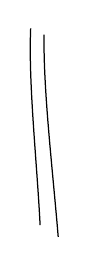
\begin{tikzpicture}[x=1mm,y=1mm,baseline=(current bounding box.north)]
\draw[line width=.45pt] (0,0) .. controls (-.3,-7) and (.8,-17) .. (1.2,-25);
\draw[line width=.45pt] (1.7,-.8) .. controls (1.6,-8) and (2.8,-18) .. (3.5,-26.5);
\end{tikzpicture}}
\deleted{ou} Demander à Quillen relations entre la notion de m-\deleted{\unsure{c|e}}Catégorie dans
la catégorie (n-Cat), et celle de ensemble (m+n)-semisimplicial.\linebreak
\deleted{(en particulier entre cette dernière notion et celle de}

L'interprétation standard semisimpliciale permet d'interpréter

\margin{37}
